\chapter{Results}
\label{chap:results}

% All main results reported at slice_2 (mid-rescripting), aggregated across
% vignettes. Full per-condition tables in Appendix D.

All results are reported at the second rewriting-turn boundary
(\techil{slice\_2}), aggregated across six vignettes. Each data point
represents the mean of twenty independent trials. Full per-condition
tables appear in Appendix~D.

\section{Plan Validity and Strategy Distribution}
\label{sec:res-validity}
% Validity rates across models and temperatures -- quality gate before
%   any stability analysis
% Strategy frequency distribution: heatmap (model x strategy category)
% [GRAPH] Validity rate per model x temperature
% [GRAPH] Strategy frequency heatmap (model x category)

Before analysing stability, the plan extraction step must be validated.
A trial is valid if the model produces a well-formed plan block containing
at least one recognised strategy category. Across all 6{,}000 trials,
validity rates exceed 99\% for every model. The lowest rates belong to
\modelname{Qwen~3.5~27B} (99.3\%) and \modelname{OLMo~3.1~32B} (99.7\%).
All other models achieve 99.8\% or above. Validity does not vary
meaningfully with temperature. These rates confirm that the fused
chain-of-thought prompt reliably elicits structured plan output, and that
the subsequent stability metrics are computed over near-complete data.

% TODO: insert Fig D.6 (validity rate) reference when appendix is written

Strategy distributions vary across models (\autoref{fig:strategy-dist}).
All ten models draw from the same six-category taxonomy, but the relative
frequencies differ. \techil{Confrontation} and \techil{self\_empowerment}
dominate across most models. \modelname{GPT-5.4} and
\modelname{Sonnet~4.6} show the narrowest distributions, concentrating on
two to three categories. \modelname{Qwen~3.5~27B} and
\modelname{Llama~3.3~70B} spread selections more evenly across categories.
These distributional differences are a prerequisite for interpreting the
consistency results that follow: a model that always selects the same two
strategies will score high on Jaccard regardless of temperature, while a
model that draws from a wider repertoire has more room to vary.

\begin{figure}[t]
  \centering
  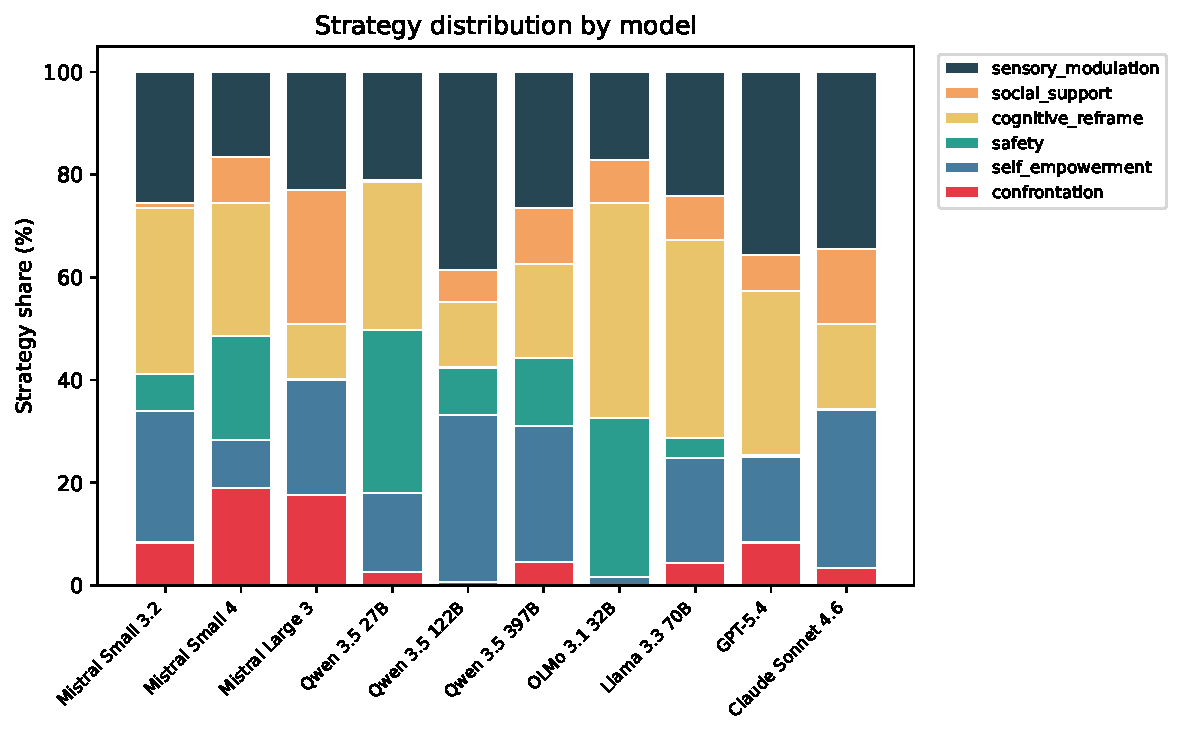
\includegraphics[width=\textwidth]{../stats/visuals_experiment/fig_5_1_strategy_distribution.pdf}
  \caption{Strategy distribution by model, pooled across temperatures and
    vignettes. Each bar shows the share of trials selecting each taxonomy
    category. Models with narrower distributions have less room to vary.}
  \label{fig:strategy-dist}
\end{figure}


% previously: Cognitive Stability (Method 1)
\section{Plan Consistency (Method 1)}
\label{sec:res-plan-consistency}
% Mean Jaccard by model x temperature -- headline figure
% Stochastic cost: degradation across temperature sweep per model
% [GRAPH] Mean Jaccard per model x temperature (bar chart)

\autoref{fig:jaccard} presents the headline result: mean Jaccard similarity
by model and temperature, grouped by model family.

\begin{figure}[t]
  \centering
  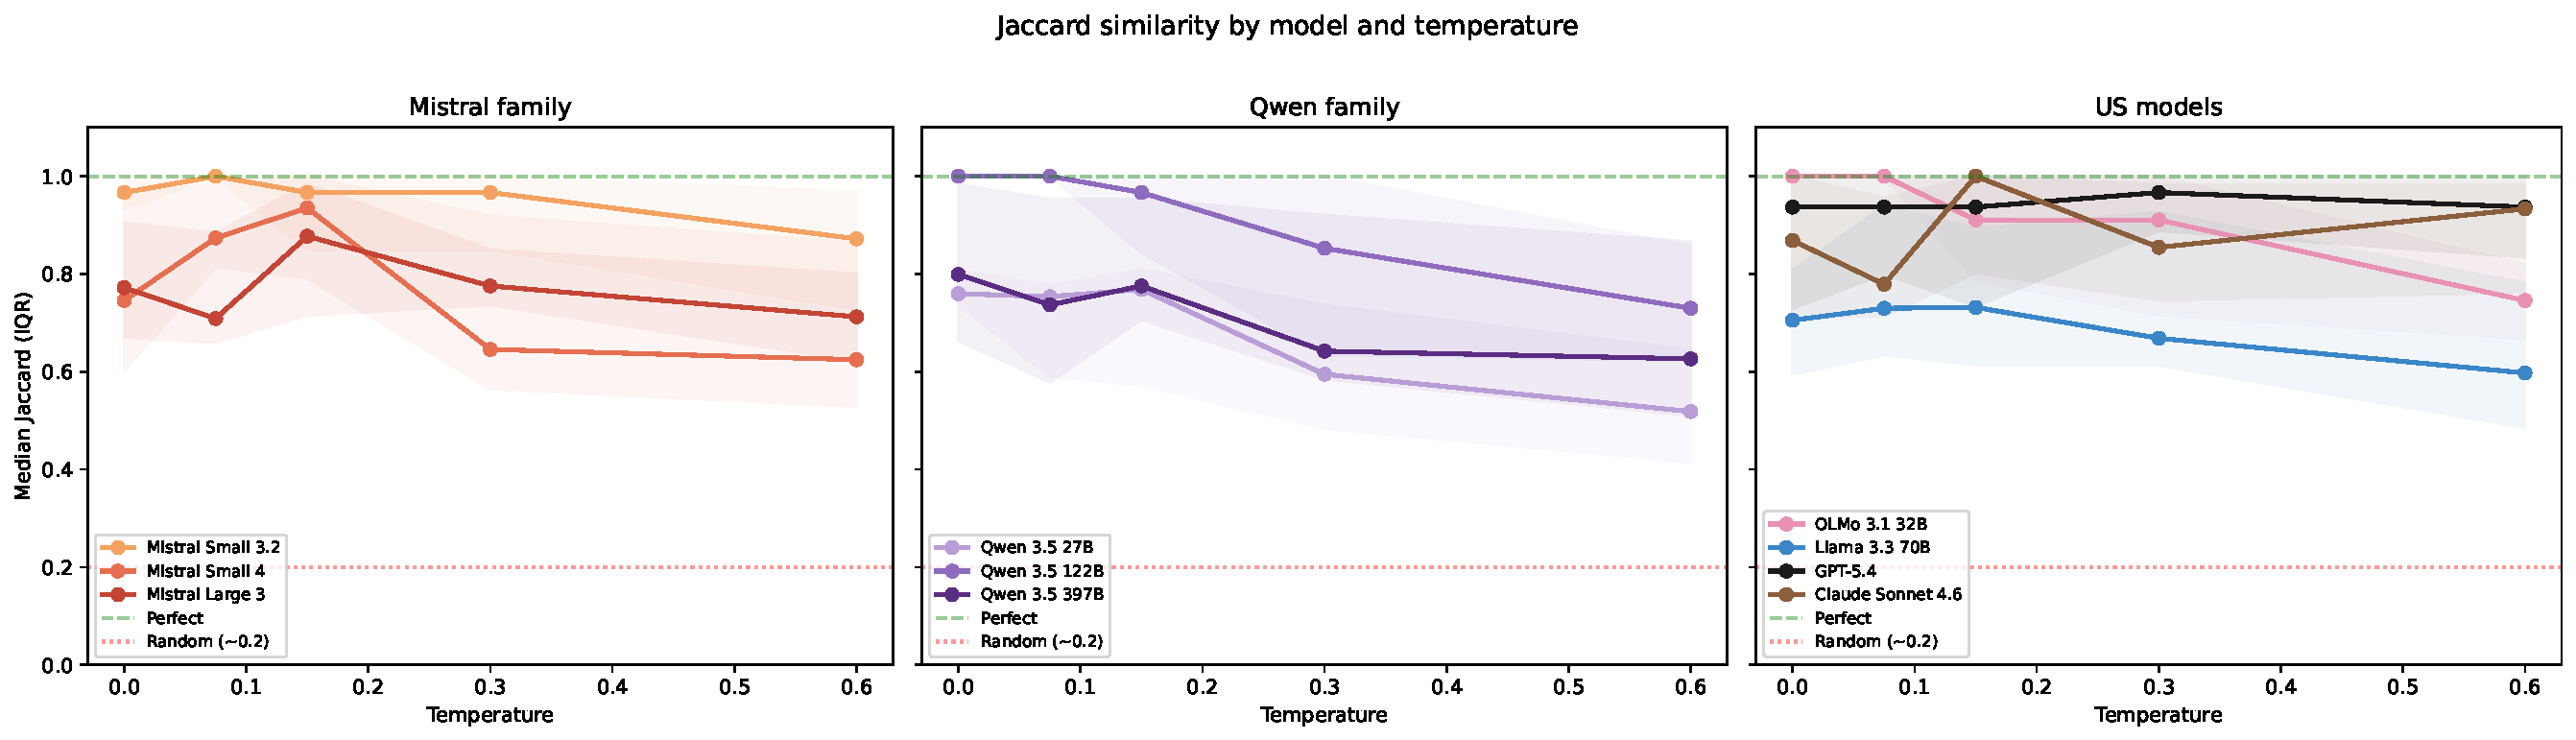
\includegraphics[width=\textwidth]{../stats/visuals_experiment/fig_5_2_jaccard.pdf}
  \caption{Mean Jaccard similarity by model and temperature, grouped by
    family. Shaded bands show $\pm 1$ SD across vignettes. The dashed
    line marks the random baseline ($J \approx 0.2$). Higher is more
    consistent.}
  \label{fig:jaccard}
\end{figure}

\paragraph{Proprietary models are temperature-immune.}
\modelname{GPT-5.4} and \modelname{Sonnet~4.6} achieve $J = 1.000$ at
every temperature point. Sampling temperature does not affect their
strategy selections at all.

\paragraph{Most open-weight models peak at low temperatures.}
The Mistral family shows a characteristic pattern:
\modelname{Mistral~Small~3.2} maintains $J = 1.000$ from $T = 0.0$
through $T = 0.3$ and drops only at $T = 0.6$ ($J = 0.933$).
\modelname{Mistral~Large~3} scores $J = 0.933$ at $T = 0.0$, rises to
$J = 1.000$ at $T = 0.075$ and $T = 0.15$, then declines to $J = 0.652$
at $T = 0.6$. \modelname{Mistral~Small~4} shows the most pronounced
version of this pattern: $J = 0.722$ at $T = 0.0$, jumping to $J = 1.000$
at $T = 0.075$ before declining.

\paragraph{Greedy decoding is not always optimal.}
Three models score higher at $T = 0.075$ than at $T = 0.0$:
\modelname{Mistral~Small~4} ($0.722 \to 1.000$),
\modelname{Mistral~Large~3} ($0.933 \to 1.000$), and
\modelname{Llama~3.3~70B} ($0.756 \to 0.881$). A small amount of sampling
variance produces more consistent strategy selection than pure greedy
decoding for these models.

\paragraph{Temperature sensitivity varies by model.}
Per-model Spearman correlations between Jaccard and temperature
(\autoref{tab:temp-spearman}) reveal three groups.
\modelname{OLMo~3.1~32B} ($\rho = -0.632$, $p < 0.001$),
\modelname{Qwen~3.5~27B} ($\rho = -0.576$, $p = 0.001$), and
\modelname{Qwen~3.5~122B} ($\rho = -0.513$, $p = 0.009$) show
statistically significant degradation. All other models, including the
entire Mistral family, show no significant temperature effect on Jaccard.
The pooled correlation across all models is $\rho = -0.228$ ($p < 0.001$).

\begin{table}[t]
  \centering
  \caption{Spearman correlation between Jaccard and temperature, per model.
    Significant correlations ($p < 0.05$) are marked with an asterisk.}
  \label{tab:temp-spearman}
  \begin{tabular}{lrrl}
    \toprule
    Model & $\rho$ & $p$ & Sig. \\
    \midrule
    Mistral Small 3.2  & $-0.190$ & 0.315 & \\
    Mistral Small 4    & $-0.196$ & 0.299 & \\
    Mistral Large 3    & $-0.277$ & 0.139 & \\
    Qwen 3.5 27B       & $-0.576$ & 0.001 & * \\
    Qwen 3.5 122B      & $-0.513$ & 0.009 & * \\
    Qwen 3.5 397B      & $-0.232$ & 0.217 & \\
    OLMo 3.1 32B       & $-0.632$ & $<$0.001 & * \\
    Llama 3.3 70B      & $-0.153$ & 0.421 & \\
    GPT-5.4            & $+0.075$ & 0.695 & \\
    Claude Sonnet 4.6  & $-0.063$ & 0.741 & \\
    \midrule
    Pooled             & $-0.228$ & $<$0.001 & * \\
    \bottomrule
  \end{tabular}
\end{table}


% previously: Output Consistency (Method 2)
\section{Response Similarity (Method 2)}
\label{sec:res-similarity}
% Mean BERTScore F1 by model x temperature -- same format as 5.2
% [GRAPH] Mean BERTScore F1 per model x temperature (bar chart)

BERTScore F1 measures semantic similarity between response texts,
independent of the plan block. The pooled temperature effect is stronger
than for Jaccard ($\rho = -0.486$, $p < 0.001$): rising temperature
changes response wording more than it changes strategy selection.

However, BERTScore has limited sensitivity to plan-level differences.
The slice depth analysis (\autoref{sec:res-secondary}) confirms this:
across conversation depths, Jaccard varies visibly while BERTScore remains
flat. A model that switches from \techil{confrontation} to
\techil{cognitive\_reframe} changes its therapeutic plan but produces
surface text similar enough that BERTScore does not detect the difference.

BERTScore therefore captures response \emph{style} consistency rather than
decision \emph{content} consistency. It serves as a sanity check: if
BERTScore were low, the model would be generating erratic text regardless
of strategy. The substantive signal for therapeutic stability comes from
Jaccard and alignment.

Full BERTScore results by model and temperature appear in Appendix~D.

% TODO: reference Fig D.2 (bertscore 3-panel) when appendix written


% previously: Plan-Output Alignment (Method 3)
\section{Plan-Response Alignment (Method 3)}
\label{sec:res-alignment}
% Mean alignment score by model x temperature
% Per-strategy scoring distributions (absent / partial / implemented)
% [GRAPH] Mean alignment per model x temperature
% [GRAPH] Stacked bar: absent / partial / implemented per strategy category

\autoref{fig:alignment} shows plan-response alignment by temperature and
per model. Alignment measures whether the model's response implements the
strategies it declared in its plan.

\begin{figure}[t]
  \centering
  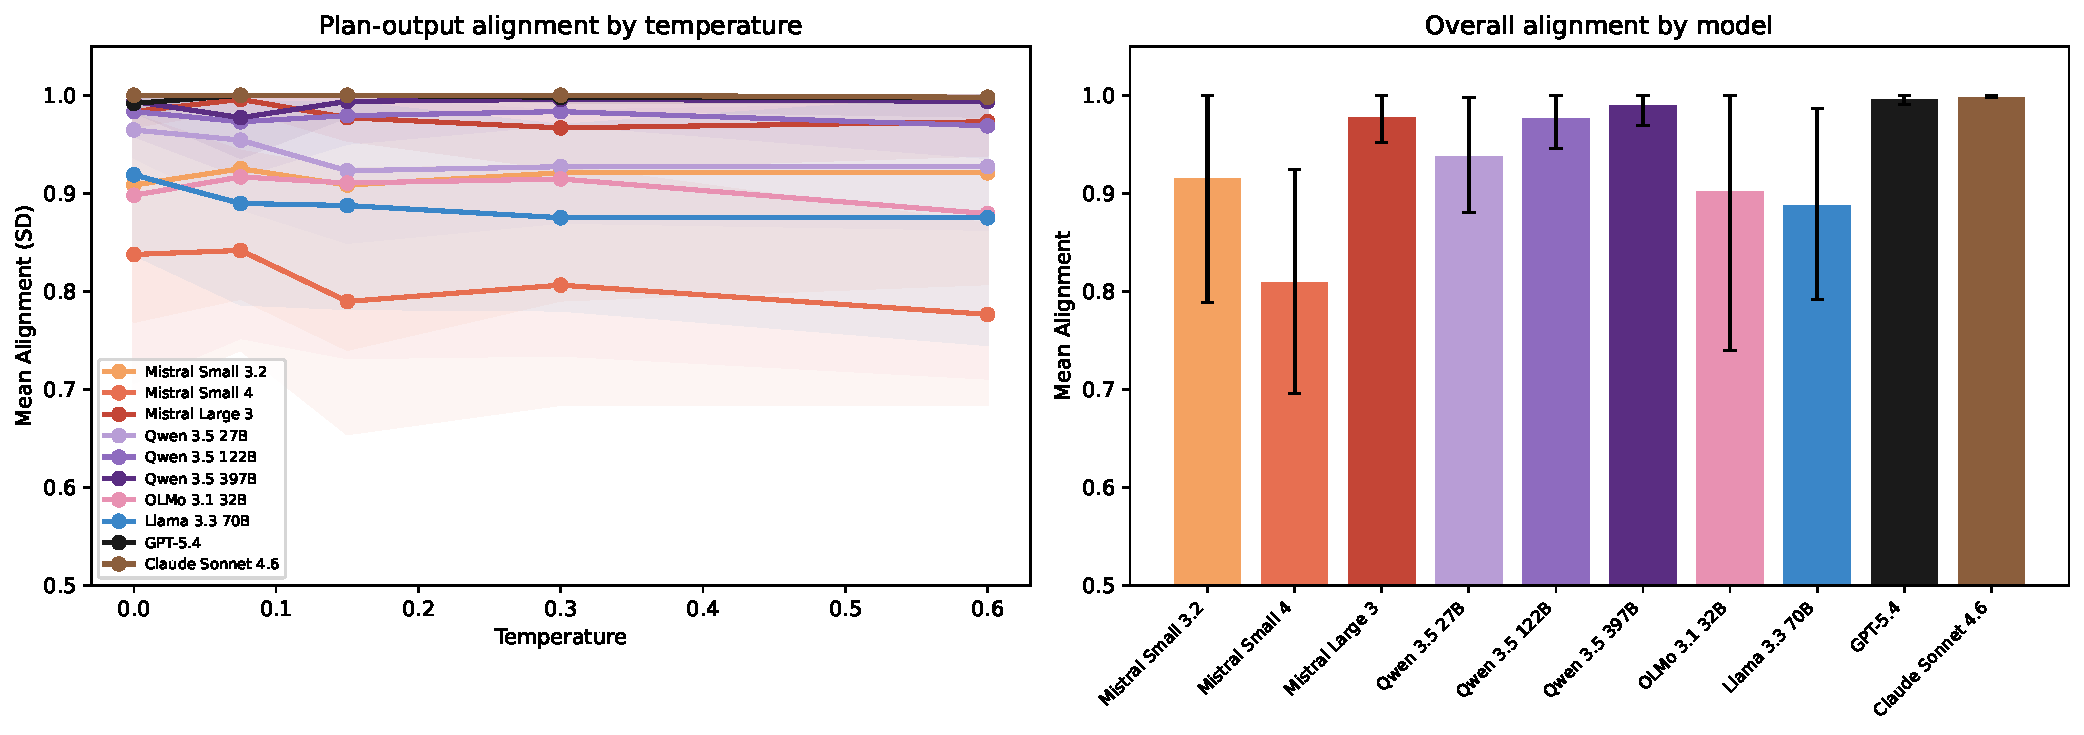
\includegraphics[width=\textwidth]{../stats/visuals_experiment/fig_5_6_alignment.pdf}
  \caption{Plan-response alignment by temperature (left) and overall by
    model (right). Error bars show $\pm 1$ SD. Most models implement their
    declared strategies consistently regardless of temperature.}
  \label{fig:alignment}
\end{figure}

The central finding is that alignment is temperature-independent. The
pooled Spearman correlation between alignment and temperature is
$\rho = -0.053$ ($p = 0.361$), not significant. Models do not get worse
at implementing their declared strategies as temperature rises. They
select \emph{different} strategies more often (lower Jaccard) but
implement whichever strategies they select equally well (stable alignment).

This dissociation has a clinical implication: temperature-induced
instability occurs at the decision-making level, not at the execution
level. A model at high temperature does not produce incoherent responses.
It produces coherent responses to a different therapeutic plan.

Kruskal-Wallis tests confirm that models differ significantly on alignment
($p < 0.001$). \modelname{Mistral~Small~4} shows the lowest mean
alignment, consistent with its erratic strategy selection at extreme
temperatures. The proprietary models and \modelname{Mistral~Small~3.2}
cluster near the top.


\section{Cross-Method Analysis}
\label{sec:res-cross}
% Spearman rank correlations: M1-M2, M1-M3, M2-M3
% Per-model stability profiles across all three methods
% Divergence cases:
%   High plan consistency + low response similarity = same strategies, variable execution
%   Low plan consistency + high response similarity = different strategies, similar surface
% [GRAPH] Correlation table (3 pairs)
% [GRAPH] Radar or grouped bar: per-model profile across all three methods

The three evaluation methods are related but not redundant.
\autoref{tab:cross-corr} reports Spearman correlations between all method
pairs, and \autoref{fig:correlations} visualises the relationship between
strategy and semantic consistency.

\begin{table}[t]
  \centering
  \caption{Spearman correlations between the three evaluation methods.
    All correlations are significant ($p < 0.001$). The moderate
    Jaccard--BERTScore correlation and weak Jaccard--Alignment correlation
    confirm that the methods capture distinct dimensions.}
  \label{tab:cross-corr}
  \begin{tabular}{lrl}
    \toprule
    Method pair & $\rho$ & Interpretation \\
    \midrule
    Jaccard \vs BERTScore   & 0.560 & Moderate \\
    Jaccard \vs Alignment   & 0.285 & Weak \\
    BERTScore \vs Alignment & 0.376 & Weak--moderate \\
    \bottomrule
  \end{tabular}
\end{table}

\begin{figure}[t]
  \centering
  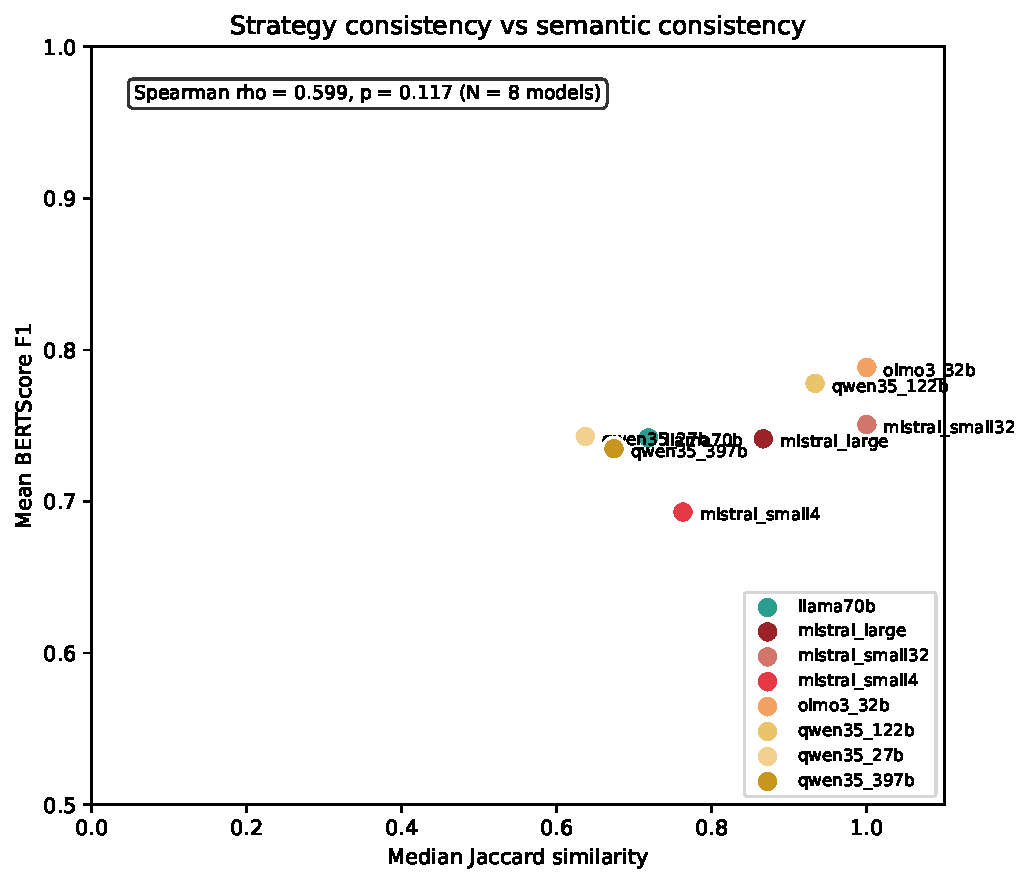
\includegraphics[width=0.7\textwidth]{../stats/visuals_experiment/fig_5_5_correlations.pdf}
  \caption{Strategy consistency (median Jaccard) versus semantic
    consistency (mean BERTScore F1) per model, pooled across temperatures.
    The proprietary models cluster in the upper-right corner.
    \modelname{Qwen~3.5~27B} and \modelname{Mistral~Small~4} occupy
    opposite ends of the BERTScore axis despite similar Jaccard ranges.}
  \label{fig:correlations}
\end{figure}

The moderate Jaccard--BERTScore correlation ($\rho = 0.560$) indicates
that models with more consistent strategy selection also tend to produce
more similar response text, but the relationship is not strong enough
for one metric to substitute for the other. The weak Jaccard--Alignment
correlation ($\rho = 0.285$) confirms that plan consistency and
plan-response coherence measure different properties.

The scatter plot (\autoref{fig:correlations}) reveals the model landscape.
\modelname{GPT-5.4} and \modelname{Sonnet~4.6} anchor the upper-right
corner: high on both dimensions. \modelname{Qwen~3.5~27B} sits in the
lower-left: low strategy consistency and low semantic similarity.
\modelname{Mistral~Small~4} presents an interesting case: moderate Jaccard
but the lowest BERTScore in the set, suggesting that even when it selects
the same strategies, its response wording varies considerably.


\section{Secondary Effects}
\label{sec:res-secondary}
% Vignette difficulty: heatmap (model x vignette) showing where instability
%   concentrates. Which patient profiles challenge consistency most?
% Conversation depth: slice_1 vs slice_3 for primary model (Mistral Large 3).
%   Early rescripting (less anchoring context) may show more variable strategy
%   selection than later turns where prior exchanges anchor the model.
% [GRAPH] Vignette heatmap (model x vignette, one per method or combined)
% [GRAPH] Slice comparison: slice_1 vs slice_2 vs slice_3 for Mistral Large

\subsection{Vignette Effects}

Kruskal-Wallis tests detect a significant vignette effect on Jaccard
($p = 0.007$) and BERTScore ($p = 0.015$). Some patient profiles produce
more consistent therapeutic responses than others across models. Full
per-vignette heatmaps appear in Appendix~D.

% TODO: reference Fig D.3 (vignette heatmaps) when appendix written

\subsection{Conversation Depth}

A preliminary analysis tested \modelname{Mistral~Large~3} at five
conversation depths (slices~1--5) across all six vignettes at $T = 0.075$
and $T = 0.15$. \autoref{fig:slice-depth} shows the results.

\begin{figure}[t]
  \centering
  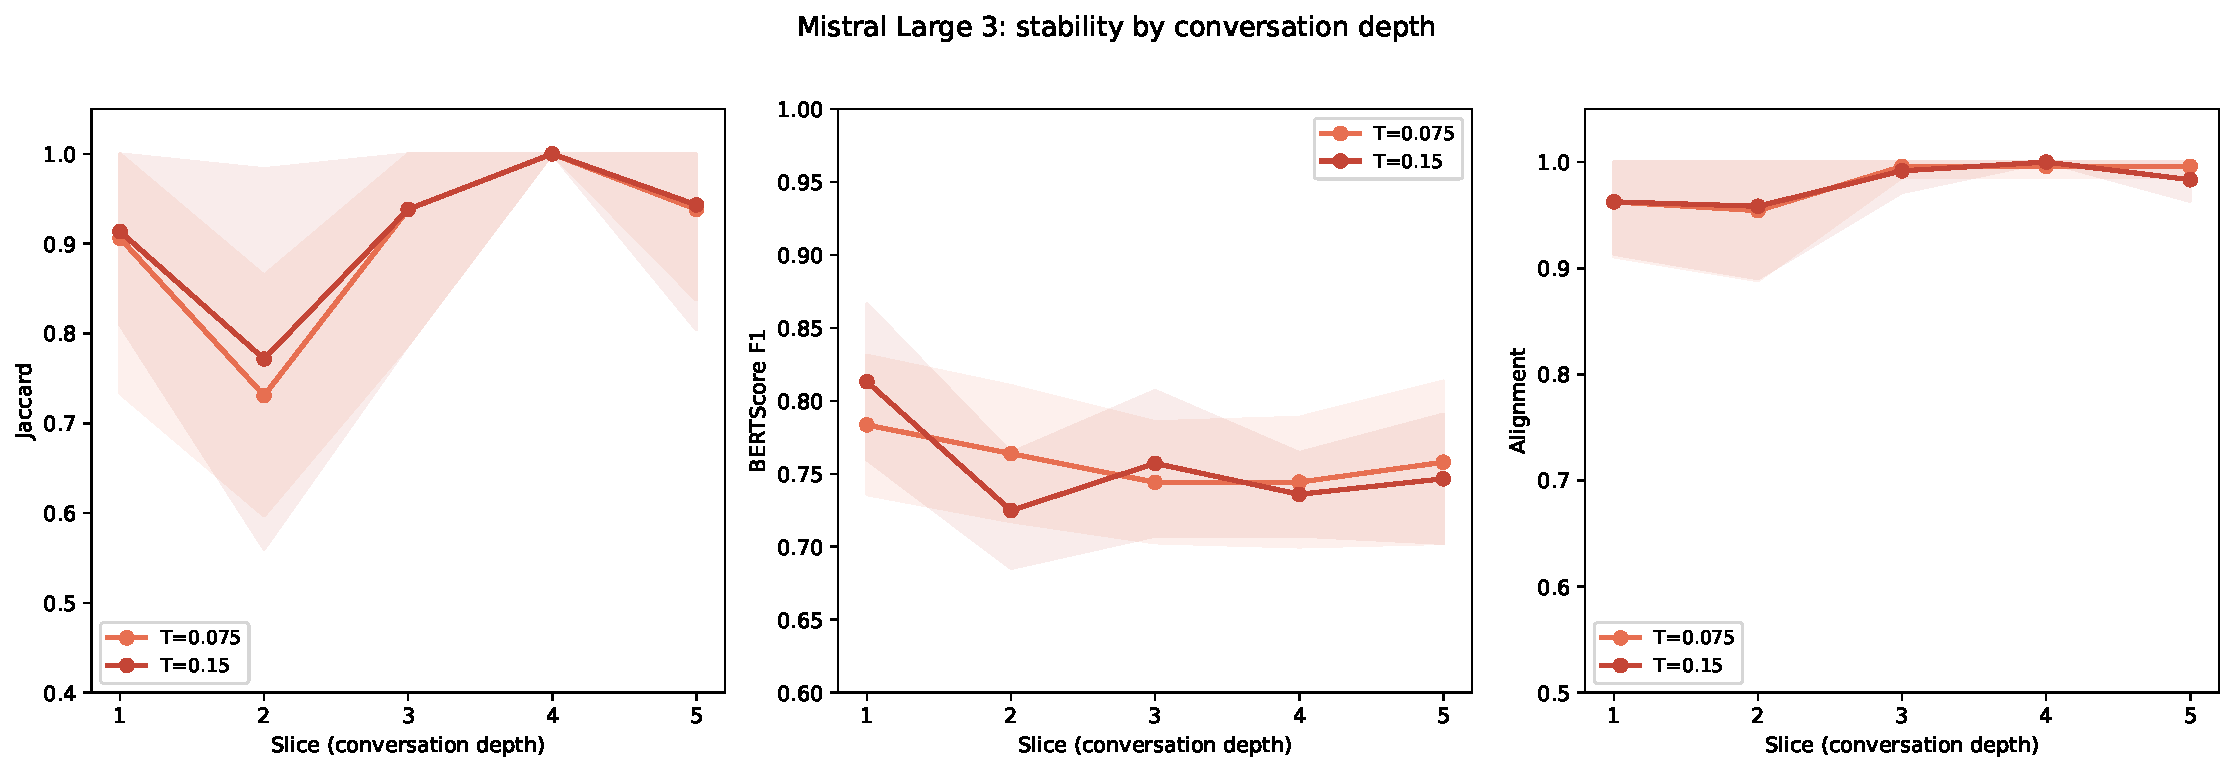
\includegraphics[width=\textwidth]{../stats/visuals_experiment/fig_slice_depth_metrics.pdf}
  \caption{Stability by conversation depth for \modelname{Mistral~Large~3}.
    Jaccard is lowest at slice~2 and rises to near-ceiling values from
    slice~3 onward. BERTScore and alignment remain flat across depths.}
  \label{fig:slice-depth}
\end{figure}

Jaccard consistency is lowest at the second slice (mean $J = 0.77$ at
$T = 0.075$) and rises to near-ceiling values from the third slice onward
($J > 0.93$). BERTScore and alignment remain flat across all depths,
confirming that conversation depth affects strategy \emph{selection} but
not response \emph{wording} or plan \emph{execution}.

The main experiment evaluates at slice~2, making the reported stability
scores a conservative estimate. A model that achieves high consistency at
this depth would likely score even higher at later conversation points
where prior exchanges provide more anchoring context.
